4. \begin{figure}[ht!]
\center{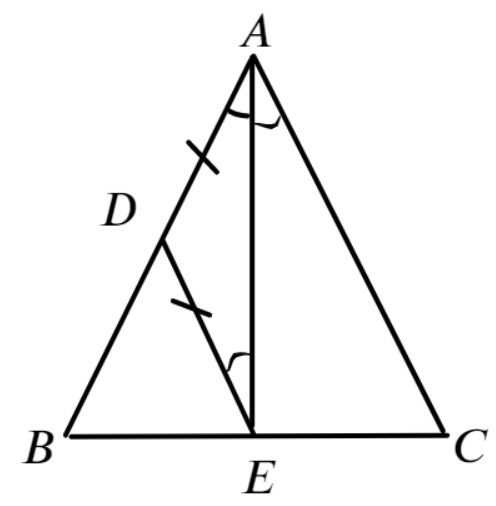
\includegraphics[scale=0.35]{g4.png}}
\end{figure}\\
Треугольник $DAE$ является равнобедренным $(AD=DE),$ значит углы при основании равны: $\angle DAE=\angle DEA.$ Прямые $DE$ и $AC$ параллельны, $AE$ секущая, значит  $\angle DEA=\angle EAC$ как накрест лежащие. Поэтому $\angle DAE=\angle EAC,$ то есть $AE$ является биссектрисой угла $A,$ а поэтому и высотой (так как треугольник $ABC$ равнобедренный). Значит, $AE\perp BC.$\\
